\subsection{Maßnahmen zur Parallelisierung}
\label{bpr:parallelisierung}

Die \bpr Variante von Schürmann und Stoye \cite{saca:2} beschreibt einen komplett sequentiellen Algorithmus zur Konstruktion von {Suf\-fix\-arrays}.
Die Autoren haben zudem nicht die Intention geäußert, den Algorithmus durch die Verwendung entsprechender Teilalgorithmen grundlegend parallelisierbar zu konzipieren.
Deshalb ist es Teil der Zielsetzung der Projektgruppe, \bpr auf Parallelisierbarkeit zu untersuchen und mit bekannten anderen Verfahren zu vergleichen.\par\smallskip
Bei genauerer Betrachtung des Algorithmus fällt auf, dass sich einige der eingesetzten Komponenten durch parallele Algorithmen ersetzen lassen, was die Laufzeit auf Multicore-Systemen positiv beeinflusst.
Andere Teile des Algorithmus hingegen sind nur für den sequentiellen Einsatz konzipiert und konnten nicht durch vergleichbare parallele Methoden ersetzt werden.

\paragraph{Bucketsort}
Die initiale Sortierung des \bpr Algorithmus geschieht in der sequentiellen Version mittels Bucketsort (\cref{section:bucketsort}).
Bucketsort selbst ist in mehrere Phasen gegliedert, von denen sich die erste und die letzte Phase parallelisieren lassen.
In der ersten Phase bestimmt Bucketsort die absoluten Häufigkeiten \(h(p)\) für alle Präfixe \(p \in \{\Sigma \cup \$\}^k\) der Länge \(k\).
Dies geschieht in der parallelen Version, indem jeder Thread \(i \in \{0, \ldots, t-1\}\) einen gleich großen Abschnitt des Eingabetextes \(\mathsf{T}\) zugewiesen bekommt und für diesen lokal die Häufigkeiten \(h_i(p)\) bestimmt.
Zentral werden daraus im Anschluss zunächst die globalen Häufigkeiten \(h(p) = \sum_{i=0}^{t-1} h_i(p)\) und darauf basierend die Startpositionen \(H(p) = \sum_{p^\prime < p} h(p^\prime)\) der Buckets im \(\mathsf{SA}\) mittels einer Präfixsumme bestimmt.
Zusätzlich zur Berechnung der Startpositionen bestimmt die parallele Variante von Bucketsort für jeden Bucket eine Thread-lokale Startposition \(H_i(p) = H(p) + \sum_{j=0}^{i-1} h_j(p)\) basierend auf den lokal gezählten Häufigkeiten des jeweiligen Elements.
In einem erneuten parallelen Scan befüllt dann jeder Thread den ihm zugewiesenen Teil jedes Buckets mit den eingelesenen Substrings der Eingabe.

\paragraph{Vergleichsbasierte Verfeinerung der Buckets}
Die vergleichsbasierte Verfeinerung zweier Buckets \bucket{p} und \bucket{q} geschieht intuitiv unabhängig voneinander, was eine hohe Parallelisierbarkeit dieser Aufgabe vermuten lässt.
Schließlich sind zu jedem Zeitpunkt alle Buckets im Suffixarray disjunkt, was ein konfliktfreies paralleles Sortieren auf Bucketebene zulassen würde.
Tatsächlich werden aber als Sortierschlüssel die Einträge des Bucket-Pointer Arrays \bptr verwendet, welche nach Abschluss jedes Sortiervorgangs aktualisiert werden.\par
Während des Sortiervorgangs auf einem Bucket \bucket{p} sind daher Lesezugriffe auf beliebige Elemente in \bptr erforderlich und nicht nur auf solche, die mit Elementen aus \bucket{p} korrespondieren.
Insbesondere kann es dabei vorkommen, dass Einträge aus \bptr gelesen werden, die zu Elementen aus \bucket{q} gehören.
Kommt es nun vor, das während eines laufenden Sortiervorgangs auf \bucket{p} der Sortiervorgang auf \bucket{q} von einem anderen Thread beendet wird, so aktualisiert dieser Thread die zu \bucket{q} gehörigen Einträge in \bptr.
Dies führt im Allgemeinen zu einer fehlerhaften Sortierung von \bucket{p}, da sich während des laufenden Vorgangs die Sortierschlüssel verändern.\par\smallskip
Um diesem unerwünschten Effekt vorzubeugen, kann jeder Thread auf einer lokalen Kopie von \bptr arbeiten.
Die Verfeinerung de Buckets ist damit konfliktfrei und folglich korrekt.
Dieser Ansatz hat allerdings neben einem deutlich erhóhten Speicherbedarf den Nachteil, dass die Verfeinerung der Sortierschlüssel nur noch dann zur Beschleunigung eines Sortiervorgangs beitragen kann, wenn dieser vom selben Thread bearbeitet wird.
Durch eine regelmäßige Synchronisation der \bptr Arrays verschiedener Threads kann letzteres Problem zwar umgangen werden, der erhöhte Synchronisationsaufwand führt allerdings durch häufiges Kopieren von Speicherinhalten zu keiner Verbesserung der Performance.
Beide Methoden zur Parallelisierung führen unter den Testbedingungen dazu, dass die parallele Variante des Algorithmus unter Verwendung dieses Verfahrens weitaus ineffizienter wird als die sequentielle Variante.\par\smallskip
Die naive Methode zur Parallelisierung ist die Verwendung eines parallelen Sortierverfahrens anstelle eines sequentiellen Verfahrens.
Die einzlenen Buckets werden auf diese Weise weiterhin sequentiell verarbeitet, der Sortiervorgang innerhalb eines Buckets profitiert aber möglicherweise von der Verwendung mehrerer Threads. Dazu wird der sequentielle IPS\(^4\)o \cite{axtmann2017} durch die entsprechende parallele Version ersetzt.
Um überflüssige Synchronisation zwischen Threads zu vermeiden, werden nur Buckets mit mehr als 5000 Elementen parallel sortiert.

%In der Referenzimplementierung verwendet Schürmann eine Version von Quicksort, um die Suffixe innerhalb der Buckets anhand ihrer Schlüssel zu sortieren. Für kleine Buckets mit einer Größe von maximal 15 Elementen wird dort Insertionsort verwendet. Einen deutlichen Vorteil gegenüber den von uns getesteten Varianten von Quicksort bietet in den meisten Fällen der Algorithmus In-Place Parallel Super Scalar Samplesort (IPS\(^4\)o \cite{axtmann2017}). Die Verwendung dieses Algorithmus hat die tatsächliche Laufzeit auf natürlichsprachlichen Eingaben von über 50\,MB ausreichend beschleunigt, um eine schnellere Verarbeitung zu ermöglichen als die Referenzimplemtierung. Bei repetitiven Texten hingegen fällt der Vorteil von Quicksort und IPS\(^4\)o deutlich geringer aus. Ein Unterschied ist hier nicht mehr messbar.

%\paragraph{Seward's copy}
%Beide Varianten des Algorithmus verwenden die von Seward \cite{seward2000} beschriebene Copy-Technik, um aus bereits sortierten Einträgen die Reihenfolge von bis dahin unsortierten Suffixen abzuleiten. 
%\begin{figure}[ht]
%	\resizebox{\textwidth}{!}{
%		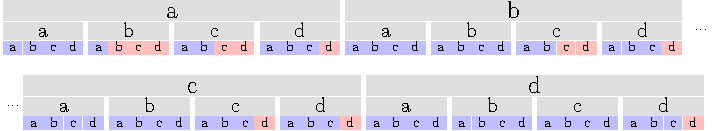
\includegraphics{kapitel/saca_algorithmen/bpr/effizienz/modifikationen/seward/image.pdf}
%	}
%    \caption[Funktionsweise der Copy-Technik]{Level-1 bis Level-3 Buckets über dem Alphabet \(\{a, b, c, d\}\). Rot markierte Buckets müssen mit Quicksort sortiert werden. Blau markierte Buckets können in Linearzeit induziert werden.}
%	\label{fig:seward}
%\end{figure}
%Der Unterschied besteht lediglich in der Reihenfolge, in der die Sortieroperationen und das Induzieren angewendet werden: Während Schürmann nach jedem Durchlauf durch einen Top-Level Bucket direkt den Rest dieses Buckets induziert und danach erneut die Bucket-Pointer aktualisiert, werden bei der \sacabench-Implementierung zuerst alle Top-Level Buckets vorsortiert, bevor im Anschluss in einem Durchlauf alle verbleibenden Indizes zusammen induziert werden. 
%\begin{listing}[h]
%    \begin{minipage}{0.5\textwidth}
%        \begin{minted}[autogobble, mathescape]{python}
%            # m is assumed to be $|\Sigma|$
%            for x in 0..m-1
%              for y in x+1..m-1
%                for z in y..m-1
%                  quicksort on bucket xyz
%                  update bucket pointers
%            for x in 0..m
%              seward-copy rest of bucket x
%        \end{minted}
%    \end{minipage}
%    \begin{minipage}{0.5\textwidth}
%        \begin{minted}[autogobble, mathescape]{python}
%            # m is assumed to be $|\Sigma|$
%            for x in 0..m-1
%              for y in x+1..m-1
%                for z in y..m-1
%                  quicksort on bucket xyz
%                  update bucket pointers
%              seward-copy rest of bucket x
%              update bucket pointers
%        \end{minted}
%    \end{minipage}
%    \caption[Verwendung der Copy Technik]{Verwendung der Copy Technik der \sacabench-Version (links) und bei Schürmann (rechts)}
%\end{listing}
%Letzteres erspart im Vergleich zur Referenzimplementierung die Aktualisierung der Bucket-Pointer nach dem Induzieren, welche als Random Access auf das Array einen messbaren Teil der Laufzeit verursachen. Die Aktualisierung kann weg fallen, da die Bucket-Pointer lediglich als Sortierschlüssel für Quicksort verwendet werden, was aber in dieser Variante zum Zeitpunkt der Induzierung schon abgeschlossen werden.\par
%Zu erwarten ist, dass bedingt durch die zum Zeitpunkt der späteren Quicksort-Aufrufe im Vergleich zur Referenzimplentierung noch ungenaueren Sortierschlüssel mehr Sortieraufrufe durchgeführt werden müssen, was eine längere Laufzeit zur Folge hat. Ein solcher Effekt war jedoch für Eingabegrößen bis zu mehreren hundert Megabyte nicht messbar.
